%%%% File:           lmsthesis.tex
%%%% Created:        2015-08-20
%%%% Modified:       2015-10-05
%%%% Author:         Dipl.-Ing. Marcus Laumer
%%%% Description:    This LaTeX template is supposed to be used for writing a thesis at the chair of
%%%%                 Multimedia Communications and Signal Processing (LMS) at the Friedrich-Alexander-Universität Erlangen-Nürnberg (FAU)

\documentclass[
paper=A4,               % paper format
pagesize=auto,          % provide page size for compiler
fontsize=12pt,          % font size
DIV=16,                 % type area calculation
twoside=true,           % two-sided layout for printing
BCOR=20mm,              % binding correction for printing (ask at copy shop!)
parskip=false,          % space between paragraphs
chapterprefix=true,     % prefix before chapter names: Chapter #
appendixprefix=true,    % prefix before appendix names: Appendix #
listof=totoc,           % include lists of figures and tables in TOC
bibliography=totoc,     % include bibliography in TOC
headinclude=true,       % header included in type area
footinclude=false,      % footer included in type area
headsepline=true,       % separation line between header and text
footsepline=false,      % separation line between footer and text
headings=small,         % size of headings
numbers=noenddot        % no dot after chapter heading prefixes
] {scrbook}

\usepackage{lmodern}
\usepackage[T1]{fontenc}
\usepackage[utf8]{inputenc}
%\usepackage[ngerman]{babel} % can be used for writing the thesis in German
\usepackage[onehalfspacing]{setspace}
\usepackage{amsmath,amssymb}
\usepackage{graphicx}
\usepackage{wrapfig}
\usepackage[caption=false]{subfig}
\usepackage{booktabs}
\usepackage[printonlyused]{acronym}
\usepackage{pdfpages}

\usepackage{blindtext} % delete in final version!

% custom packages
\usepackage[backref=page]{hyperref}
% for backreference with arrow
\renewcommand\backrefxxx[3]{%
  \hyperlink{page.#1}{$\uparrow$#1}%
}

\graphicspath{{figures/}}

\recalctypearea

\begin{document}

    \pagenumbering{Alph} % will not be displayed
    \begin{titlepage}
    \vspace*{6ex}
    \begin{center}
        \LARGE
        Friedrich-Alexander-Universität Erlangen-Nürnberg\\[1.5ex]
        \Large
        \textbf{Lehrstuhl für Multimediakommunikation und Signalverarbeitung}\\[1.5ex]
        Prof. Dr.-Ing. André Kaup\\
        \vfill
        \LARGE
        Master Thesis\\[3ex]
        \textbf{Text Recognition Algorithms for Screen Content Quality Assessment}\\[3ex]
        Sebastian Hirt\\
        \vfill
        \Large
        July 2023\\[1.5ex]
        \begin{tabular}{ll}
            Supervisors: & Prof. Dr.-Ing. André Kaup \\
            & M. Sc. Hannah Och
        \end{tabular}
    \end{center}
\end{titlepage}

    \cleardoublepage
    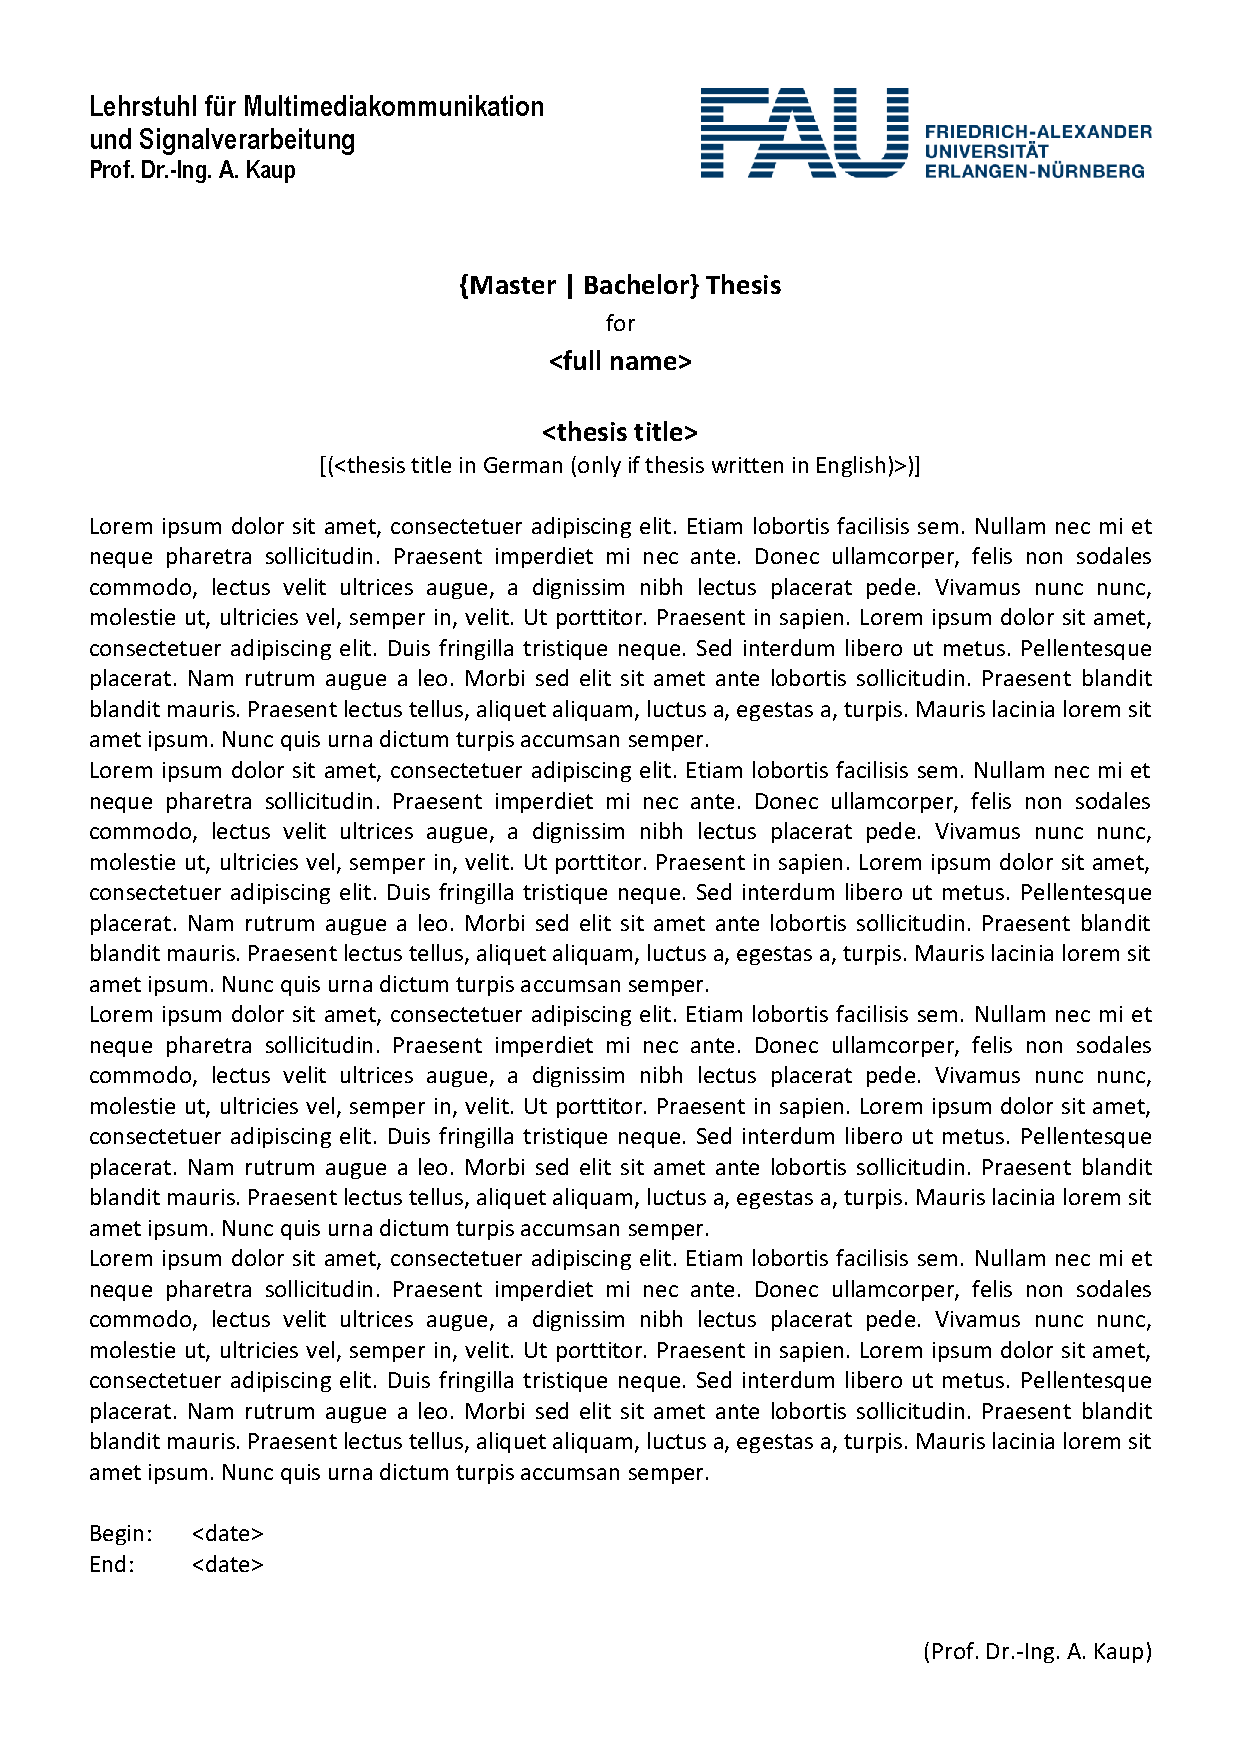
\includepdf[pages={1},scale={0.95}]{topic/topic}
    \cleardoublepage
    
    %\chapter*{Erklärung}
\thispagestyle{empty}

\noindent
Ich versichere, dass ich die vorliegende Arbeit ohne fremde Hilfe und ohne Benutzung anderer als der angegebenen Quellen angefertigt habe, und dass die Arbeit in gleicher oder ähnlicher Form noch keiner anderen Prüfungsbehörde vorgelegen hat und von dieser als Teil einer Prüfungsleistung angenommen wurde.
Alle Ausführungen, die wörtlich oder sinngemäß übernommen wurden, sind als solche gekennzeichnet.

\vspace{3cm}

\begin{minipage}[t]{0.45\textwidth}
    \rule{\textwidth}{0.5pt}\\
	Ort, Datum
\end{minipage}
\hfill
\begin{minipage}[t]{0.45\textwidth}
	\rule{\textwidth}{0.5pt}\\
	<Vollständiger Name>\\
    <Adresse>
\end{minipage}

    % or
    \chapter*{Declaration}
\thispagestyle{empty}

\noindent
I confirm that I have written this thesis unaided and without using sources other than those listed and that this thesis has never been submitted to another examination authority and accepted as part of an examination achievement, neither in this form nor in a similar form.
All content that was taken from a third party either verbatim or in substance has been acknowledged as such.

\vspace{3cm}

\begin{minipage}[t]{0.45\textwidth}
    \rule{\textwidth}{0.5pt}\\
	Erlangen, \today
\end{minipage}
\hfill
\begin{minipage}[t]{0.45\textwidth}
	\rule{\textwidth}{0.5pt}\\
	Sebastian Hirt\\
    Ellingen, Rennfeld 5b
\end{minipage}


    \frontmatter
    \pagenumbering{Roman}
    \tableofcontents
    \chapter{Kurzfassung}

In dieser Arbeit wird die Anwendung von Texterkennungsalgorithmen für die Bewertung der Bildqualität von Bildschirminhalten untersucht.
Durch die Untersuchung modernster Texterkennungs- und -erkennungsmethoden, die Erstellung eines markierten Datensatzes und die Untersuchung der Korrelation zwischen Texterkennungsraten und menschlicher Beurteilung wird eine wertvolle Ergänzung zur aktuellen Forschung geliefert.

    \chapter{Abstract}

In this thesis, the application of text recognition algorithms for the assessment of screen content image quality is explored.
By researching state-of-the-art text recognition and detection methods, generating a labeled dataset, and investigating the correlation between text recognition rates and human judgement, a valuable addition to current research is provided.

    % \chapter{Symbols and Notations}

% In order of appearance.\\

% \begin{tabular}{ll}
% +					&	Addition\\
% \end{tabular}
% \makenoidxglossaries

\newglossaryentry{add}
{
    type={symbols},
    name={+},
    description={Addition}
}

\newglossaryentry{sub}
{
    type={symbols},
    name={-},
    description={Subtraction}
}

    % old version of acronyms.tex
% \chapter{Abbreviations and Acronyms}

% In alphabetical order.

% \begin{acronym}
%     \acro{e.g.}{exempli gratia}
%     \acro{TER}{text error rate}
%     \acro{MOS}{mean opinion score}
% \end{acronym}

\newacronym{ocr}{OCR}{optical character recognition}
\newacronym{cer}{CER}{character error rate}
\newacronym{mos}{MOS}{mean opinion score}
\newacronym{psnr}{PSNR}{peak signal-to-noise ratio}
\newacronym{mse}{MSE}{mean squared error}
\newacronym{bdrate}{BDRate}{Bjøntegaard Delta Rate}
\newacronym{hevc}{HEVC}{High Efficiency Video Coding}
\newacronym{vvc}{VVC}{Versatile Video Coding}
\newacronym{scid}{SCID}{Screen Content Image Database}
\newacronym{gt}{GT}{ground truth}


    \mainmatter
    \chapter{Introduction}
\label{chap:Introduction}

\section{Motivation}

In today’s digital age, screen content plays a vital role in our daily lives.
From office work to entertainment, we are constantly interacting with images and videos on screens.
Many of these images contain text, graphics and user interface elements that are not found in natural images.
As such, the quality of screen content is of utmost importance for the viewer.
One key aspect of screen content quality is the readability of text.
However, conventional objective image quality assessment algorithms do not directly consider text readability.
This is where text recognition algorithms come into play.

In this thesis, we will explore the application of text recognition algorithms for the assessment of screen content image quality.
By researching state-of-the-art text recognition and detection methods, generating a labeled dataset, and investigating the correlation between text recognition rates and human judgement, we aim to provide a valuable addition to conventional quality metrics.

Through a structured implementation and detailed documentation of the framework and experiments, this thesis will provide valuable insights into the potential of text recognition algorithms for screen content quality assessment.
In this thesis, I use the pronouns \textit{we} and \textit{our} to refer to myself and the larger scientific community.

\section{Research Objectives}

--- Figure out if text recognition algorithms can be used to assess the quality of screen content images.

\section{Thesis Outline}

--- do this last

First we will give an overview of the current state of the art in text recognition and detection in \autoref{chap:related_work}.
Then we will describe the methodology used in this thesis in \autoref{chap:methods}.
Afterwards, we will present the results of our experiments in \autoref{chap:evaluation}.
Finally, we will summarize and conclude our findings in \autoref{chap:conclusion}.


    \chapter{Examples}
\label{chap:Examples}

\section{Figures}
\label{sec:Figures}

\blindtext
This is illustrated in Figure~\ref{fig:samplefigure}.

\begin{figure}[t]
    \centering
    %\includegraphics[width=0.99\textwidth]{figure}
    \rule{0.99\textwidth}{5cm}
    \caption{Sample figure with caption below.}
    \label{fig:samplefigure}
\end{figure}

\Blindtext
\blindtext
% Please refer to Figures~\ref{subfig:samplesubfigure1}, \ref{subfig:samplesubfigure2}, \ref{subfig:samplesubfigure3}, and \ref{subfig:samplesubfigure4}.

% \begin{figure}[t]
%   \centering
%   \subfloat[Caption a]{\rule{0.22\textwidth}{2cm}\label{subfig:samplesubfigure1}}\quad
%   \subfloat[Caption b]{\rule{0.22\textwidth}{2cm}\label{subfig:samplesubfigure2}}\quad
%   \subfloat[Caption c]{\rule{0.22\textwidth}{2cm}\label{subfig:samplesubfigure3}}\quad
%   \subfloat[Caption d]{\rule{0.22\textwidth}{2cm}\label{subfig:samplesubfigure4}}
%   \caption{Caption for all subfigures.}
%   \label{fig:samplesubfigures}
% \end{figure}


\section{Tables}
\label{sec:Tables}

\blindtext
Results can be found in Table~\ref{tab:sampletable}.

\begin{table}[t]
    \caption{Sample table with caption above.}
    \centering
    \begin{tabular}{ccc}
        \toprule
        Column 1    &   Column 2    &   Column 3\\
        \midrule
        One         &   Two         &   Three\\
        Un          &   Deux        &   Trois\\
        Eins        &   Zwei        &   Drei\\
        \bottomrule
    \end{tabular}
    \label{tab:sampletable}
\end{table}

\Blindtext

\section{Equations}
\label{sec:Equations}

\blindtext
Hence, the energy \(E\) is defined as
\begin{equation}
    E = mc^2 \text{ .}
    \label{eq:sampleequation}
\end{equation}
Thereby, the kinetic energy \(E_k\) of a moving object is defined as follows.
\begin{equation}
    \begin{aligned}
        E_k &= m_0\left(\gamma - 1\right) c^2 =\\
        &= \frac{m_0 c^2}{\sqrt{1 - \frac{v^2}{c^2}}} - m_0 c^2
    \end{aligned}
\end{equation}
Furthermore, the total momentum \(P\) of a particle and the relativistic mass \(m\) are:
\begin{align}
    P &= \frac{m_0 v}{\sqrt{1 - \frac{v^2}{c^2}}}\\
    m &= \frac{m_0}{\sqrt{1 - \frac{v^2}{c^2}}}
\end{align}

\Blindtext
 % delete in final version!
    %%%% insert your chapters here %%%%
    %%%% make sure that included files are encoded in UTF-8 %%%%

    \chapter{Conclusion}
\label{chap:conclusion}

In this thesis, we investigate the potential of using \gls{ocr} methods for screen content \gls{iqa}.
We compare the performance of two \gls{ocr} algorithms, EasyOCR and Tesseract \gls{ocr}, on the \gls{scid} dataset, see \autoref{sec:ocr_performance}.
First, we conclude, that both \gls{ocr} methods perform worse on the images affected by \gls{mb} and \gls{gb}, with Tesseract \gls{ocr} performing really poor for \gls{gn} as well.
However, both \gls{ocr} algorithms perform without impairment for \gls{cc}, \gls{cqd} and \gls{csc}.
Generally, the results show that both \gls{ocr} methods perform differently for different distortions, but EasyOCR performs better than Tesseract \gls{ocr}.


Subsequently, we compare the $\text{CER}_{\text{c}}$ produced by the \gls{ocr} methods to human judgment, see \autoref{sec:comparison_with_human_judgment}.
We conclude that EasyOCR is generally better suited as a estimation of human judgment compared to Tesseract \gls{ocr}.
For blurred images, EasyOCR exhibits a high correlation with human judgment.
Our recommendation is to determine if \gls{ocr} methods are affected by specific distortions or check which distortions appear in the used data before adding \gls{ocr} as a metric.
Compared to other \gls{iqa} methods, both \gls{ocr} algorithms are subpar, especially considering that we selected specifically suited images from the dataset compared to other methods being evaluated on the full dataset.
However, our method only uses the text regions of the images, which are missing a lot of information about distortion impacts on the graphical or natural parts of the image.
Thus, we recommend combining \gls{ocr} with other metrics, like the \gls{ssim} or the \gls{fsim}, to get a more complete picture of the image quality.

Additionally, we surmise that in general EasyOCR performs better than Tesseract \gls{ocr} on the reference images, but both seem to be too inaccurate to be used as true \gls{gt}, see \autoref{sec:usage_of_recognized_text_as_ground_truth}.
Finally, we investigate the performance of the \gls{ocr} methods for several \glspl{qp} of the \gls{hevc} and \gls{vvc} codecs and calculate the \glspl{bdrate} between them to compare the true \gls{gt} with the pseudo \gls{gt}.
We found EasyOCR to be a decent choice for the pseudo \gls{gt}, especially for the default codec configuration.

For future research, we recommend combining the \gls{cer} with a metric such as the \gls{iou} between hand labeled text regions and the prediction bounding boxes.
While this may involve significant amount of labeling work, it might lead to a more consistent metric as the order of the text elements becomes less relevant.
Thus, it can be used to compare different \gls{ocr} algorithms more objectively.
Moreover, the resulting regions that are not occupied by text elements could be evaluated by other more suitable metrics for pictorial regions, and then combined with the \gls{cer} into one unified metric.
Additionally, using preprocessing steps to alter the performance of the \gls{ocr} methods and improve the correlation with the \gls{mos} might be an interesting research direction.



    \appendix
    \chapter{First Appendix}
\label{chap:FirstAppendix}

Appendix (optional).


    \backmatter
    \listoffigures
    \listoftables
    \bibliographystyle{IEEEtran}
    \bibliography{bibfiles/references}
    \chapter*{Curriculum Vitae}
\thispagestyle{empty}

\begin{wrapfigure}{r}{3.5cm}
    %\includegraphics[width=3.5cm]{photo}
    \rule{3.5cm}{4.5cm}
\end{wrapfigure}

Short CV of the author.
\blindtext

\end{document}
